% Options for packages loaded elsewhere
\PassOptionsToPackage{unicode}{hyperref}
\PassOptionsToPackage{hyphens}{url}
\PassOptionsToPackage{dvipsnames,svgnames*,x11names*}{xcolor}
%
\documentclass[
]{article}
\usepackage{amsmath,amssymb}
\usepackage{lmodern}
\usepackage{ifxetex,ifluatex}
\ifnum 0\ifxetex 1\fi\ifluatex 1\fi=0 % if pdftex
  \usepackage[T1]{fontenc}
  \usepackage[utf8]{inputenc}
  \usepackage{textcomp} % provide euro and other symbols
\else % if luatex or xetex
  \usepackage{unicode-math}
  \defaultfontfeatures{Scale=MatchLowercase}
  \defaultfontfeatures[\rmfamily]{Ligatures=TeX,Scale=1}
\fi
% Use upquote if available, for straight quotes in verbatim environments
\IfFileExists{upquote.sty}{\usepackage{upquote}}{}
\IfFileExists{microtype.sty}{% use microtype if available
  \usepackage[]{microtype}
  \UseMicrotypeSet[protrusion]{basicmath} % disable protrusion for tt fonts
}{}
\makeatletter
\@ifundefined{KOMAClassName}{% if non-KOMA class
  \IfFileExists{parskip.sty}{%
    \usepackage{parskip}
  }{% else
    \setlength{\parindent}{0pt}
    \setlength{\parskip}{6pt plus 2pt minus 1pt}}
}{% if KOMA class
  \KOMAoptions{parskip=half}}
\makeatother
\usepackage{xcolor}
\IfFileExists{xurl.sty}{\usepackage{xurl}}{} % add URL line breaks if available
\IfFileExists{bookmark.sty}{\usepackage{bookmark}}{\usepackage{hyperref}}
\hypersetup{
  pdftitle={Tarea Bloque 3},
  pdfauthor={Jose Antonio Lorencio Abril},
  colorlinks=true,
  linkcolor=green,
  filecolor=Maroon,
  citecolor=Blue,
  urlcolor=Blue,
  pdfcreator={LaTeX via pandoc}}
\urlstyle{same} % disable monospaced font for URLs
\usepackage[margin=1in]{geometry}
\usepackage{graphicx}
\makeatletter
\def\maxwidth{\ifdim\Gin@nat@width>\linewidth\linewidth\else\Gin@nat@width\fi}
\def\maxheight{\ifdim\Gin@nat@height>\textheight\textheight\else\Gin@nat@height\fi}
\makeatother
% Scale images if necessary, so that they will not overflow the page
% margins by default, and it is still possible to overwrite the defaults
% using explicit options in \includegraphics[width, height, ...]{}
\setkeys{Gin}{width=\maxwidth,height=\maxheight,keepaspectratio}
% Set default figure placement to htbp
\makeatletter
\def\fps@figure{htbp}
\makeatother
\setlength{\emergencystretch}{3em} % prevent overfull lines
\providecommand{\tightlist}{%
  \setlength{\itemsep}{0pt}\setlength{\parskip}{0pt}}
\setcounter{secnumdepth}{-\maxdimen} % remove section numbering
\usepackage[utf8]{inputenc}
\usepackage{hyperref}
\usepackage{multirow}
\usepackage{float}
\ifluatex
  \usepackage{selnolig}  % disable illegal ligatures
\fi
\newlength{\cslhangindent}
\setlength{\cslhangindent}{1.5em}
\newlength{\csllabelwidth}
\setlength{\csllabelwidth}{3em}
\newenvironment{CSLReferences}[2] % #1 hanging-ident, #2 entry spacing
 {% don't indent paragraphs
  \setlength{\parindent}{0pt}
  % turn on hanging indent if param 1 is 1
  \ifodd #1 \everypar{\setlength{\hangindent}{\cslhangindent}}\ignorespaces\fi
  % set entry spacing
  \ifnum #2 > 0
  \setlength{\parskip}{#2\baselineskip}
  \fi
 }%
 {}
\usepackage{calc}
\newcommand{\CSLBlock}[1]{#1\hfill\break}
\newcommand{\CSLLeftMargin}[1]{\parbox[t]{\csllabelwidth}{#1}}
\newcommand{\CSLRightInline}[1]{\parbox[t]{\linewidth - \csllabelwidth}{#1}\break}
\newcommand{\CSLIndent}[1]{\hspace{\cslhangindent}#1}

\title{Tarea Bloque 3}
\usepackage{etoolbox}
\makeatletter
\providecommand{\subtitle}[1]{% add subtitle to \maketitle
  \apptocmd{\@title}{\par {\large #1 \par}}{}{}
}
\makeatother
\subtitle{Desarrollo de Sistemas Inteligentes}
\author{Jose Antonio Lorencio Abril}
\date{Diciembre de 2021}

\begin{document}
\maketitle

\newpage

\newpage

\hypertarget{problema-1}{%
\section{Problema 1}\label{problema-1}}

\index{Problema 1} Supongamos que para una cierta aplicación definimos
unos conjuntos borrosos con estas funciones de pertenencia:
\[\mu_{A}\left(x\right)=\frac{1}{1+e^{-2\left(x-4\right)}}\]
\[\mu_{B}\left(x\right)=\frac{1}{1+e^{3\left(x-5\right)}}\] definidos
sobre el universo \(X=\left[0,10\right]\). Calcular, analítica y
gráficamente, la unión, la intersección, los complementos, las
diferencias, las dos leyes de Morgan, la ley del medio excluido y la ley
de la contradicción.

Para la resolución de este ejercicio, seguimos las definiciones
proporcionadas en los apuntes de clase
~{[}\protect\hyperlink{ref-PalmaConjuntosBorrosos}{1}{]}, así como los
ejemplos resueltos
~{[}\protect\hyperlink{ref-BotiaConjuntosBorrosos}{2}{]}. Primero,
notamos que los conjuntos asociados a estas relaciones de pertenencia
son:
\[A=\int_{x\in\left[0,10\right]}\mu_{A}\left(x\right)/x=\int_{x\in\left[0,10\right]}\frac{1}{1+e^{-2\left(x-4\right)}}/x\]
\[B=\int_{x\in\left[0,10\right]}\mu_{B}\left(x\right)/x=\int_{x\in\left[0,10\right]}\frac{1}{1+e^{3\left(x-5\right)}}/x\]
Que tienen la siguiente pinta:

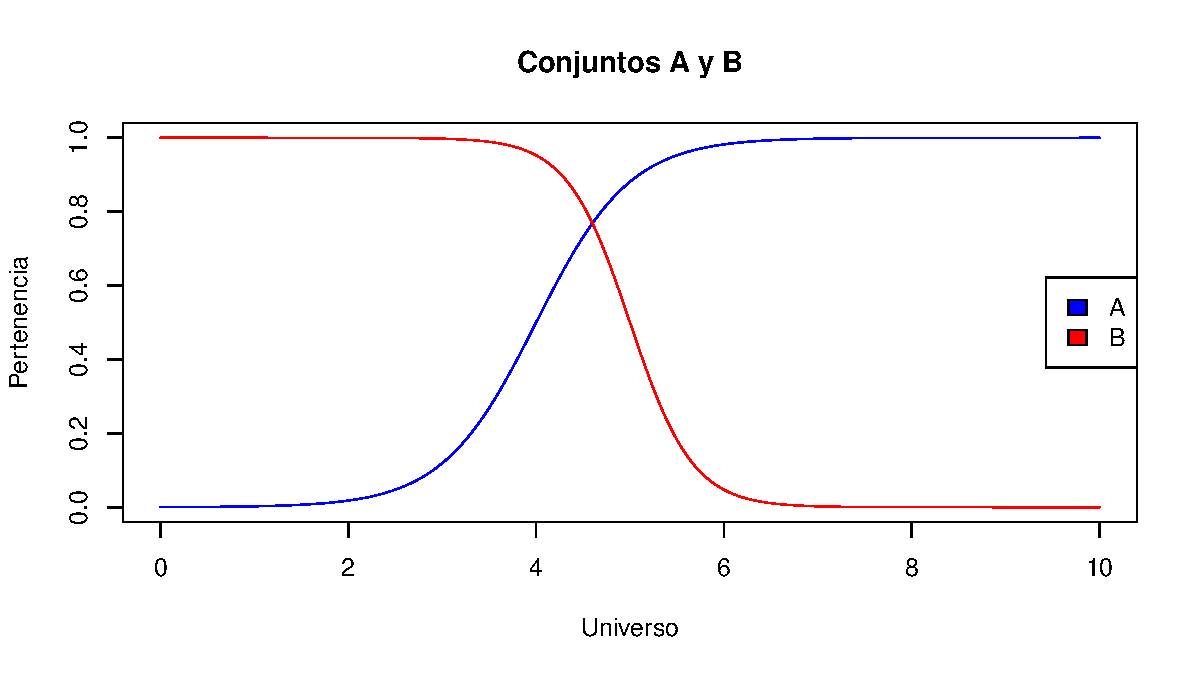
\includegraphics{tareaB3_files/figure-latex/unnamed-chunk-1-1.pdf}
\newpage Para calcular la \textbf{unión}, basta tomar el máximo de
ambas, gráficamente queda:

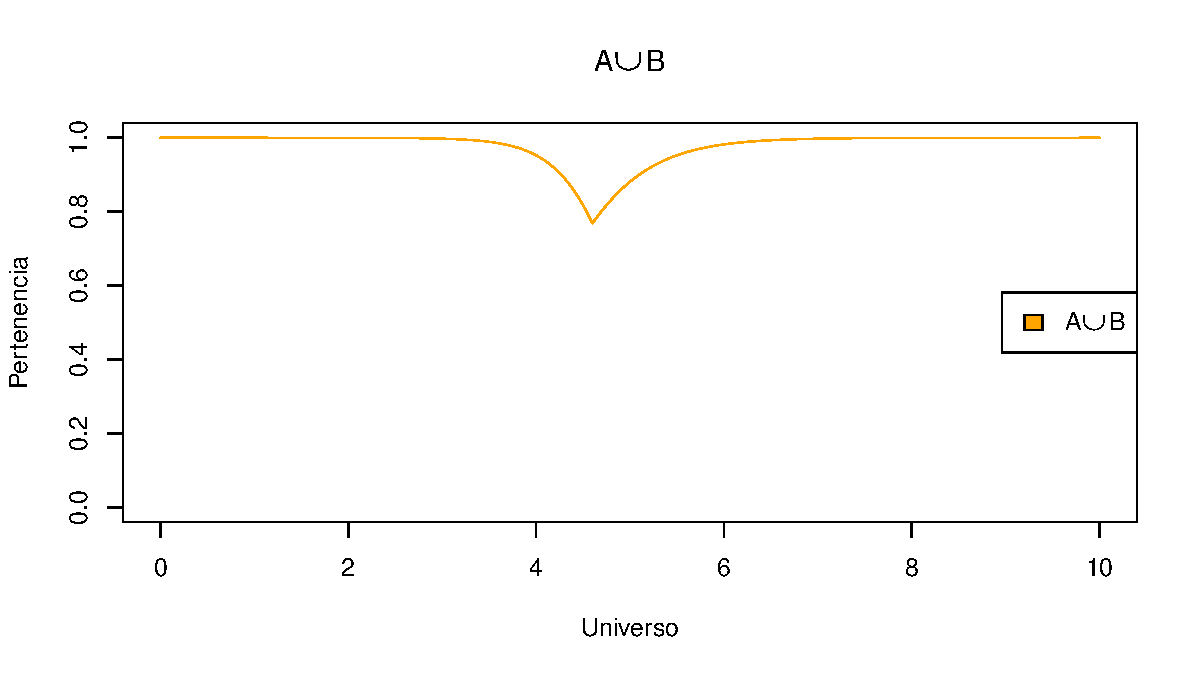
\includegraphics{tareaB3_files/figure-latex/unnamed-chunk-2-1.pdf} Para
hacerlo analíticamente:

\[\mu_{A}\left(x\right)\geq\mu_{B}\left(x\right)\iff\frac{1}{1+e^{-2\left(x-4\right)}}\geq\frac{1}{1+e^{3\left(x-5\right)}}\iff e^{-2\left(x-4\right)}\leq e^{3\left(x-5\right)}\iff\]
\[\iff-2\left(x-4\right)\leq3\left(x-5\right)\iff x-4\geq-\frac{3}{2}\left(x-5\right)\iff\frac{5}{2}x\geq\frac{23}{2}\iff x\geq\frac{23}{5}\]

Por tanto, es \[\mu_{A\cup B}\left(x\right)=\begin{cases}
\mu_{B}\left(x\right) & x\leq\frac{23}{5}\\
\mu_{A}\left(x\right) & x>\frac{23}{5}
\end{cases}\]

Para la \textbf{intersección}, lo que hacemos es el mínimo, que es igual
que antes, pero tomando la función recíproca:
\[\mu_{A\cap B}\left(x\right)=\begin{cases}
\mu_{A}\left(x\right) & x\leq\frac{23}{5}\\
\mu_{B}\left(x\right) & x>\frac{23}{5}
\end{cases}\]

De forma visual:

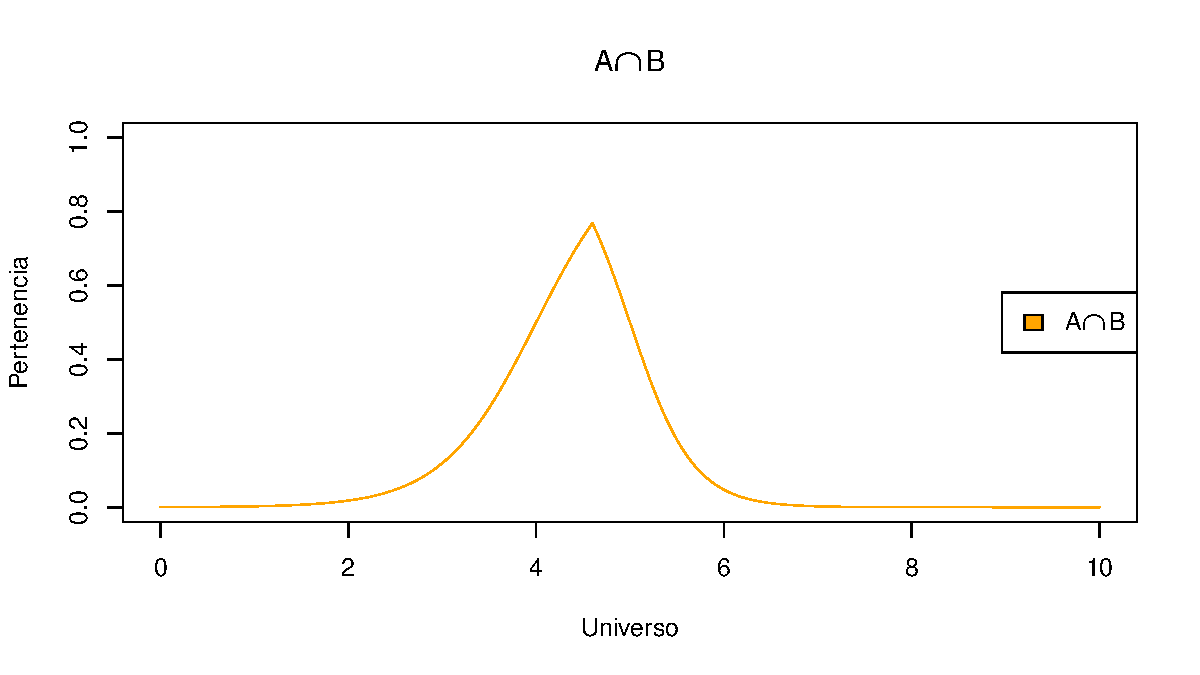
\includegraphics{tareaB3_files/figure-latex/unnamed-chunk-3-1.pdf}

Para el \textbf{complementario} simplement hay que tomar las funciones
de pertenencia complementarias, es decir
\[\mu_{\overline{A}}\left(x\right)=1-\mu_{A}\left(x\right)=1-\frac{1}{1+e^{-2\left(x-4\right)}}=\frac{e^{-2\left(x-4\right)}}{1+e^{-2\left(x-4\right)}}=\frac{1}{e^{2\left(x-4\right)}+1}=\frac{1}{1+e^{2\left(x-4\right)}}\]
\[\mu_{\overline{B}}\left(x\right)=1-\mu_{B}\left(x\right)=1-\frac{1}{1+e^{3\left(x-5\right)}}=\frac{e^{3\left(x-5\right)}}{1+e^{3\left(x-5\right)}}=\frac{1}{e^{-3\left(x-5\right)}+1}=\frac{1}{1+e^{-3\left(x-5\right)}}\]
y gráficamente:

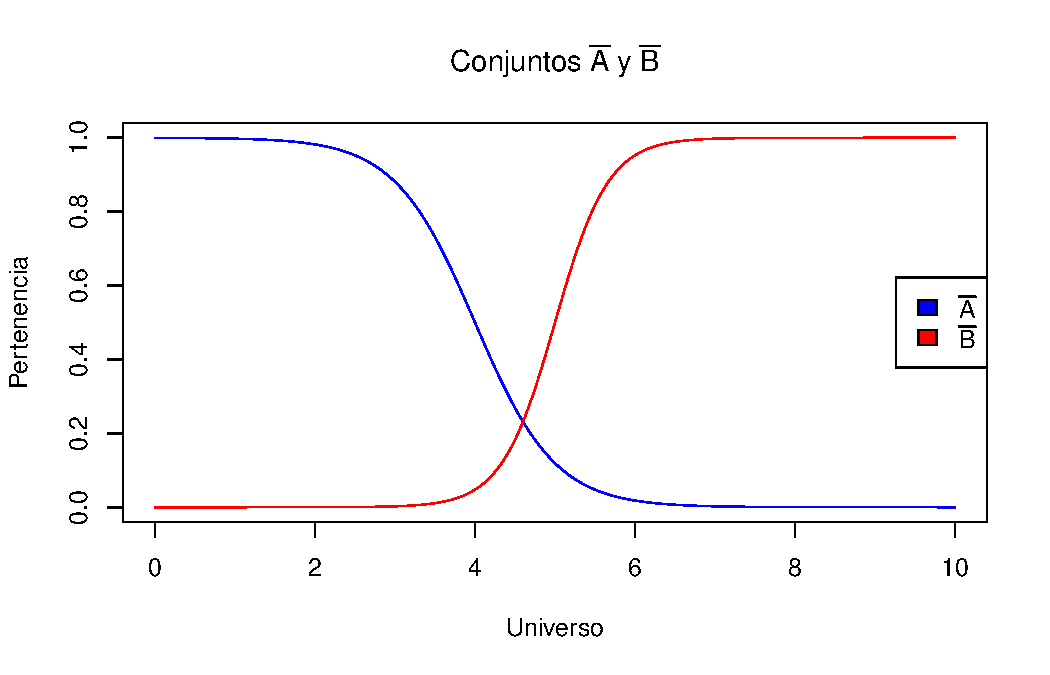
\includegraphics{tareaB3_files/figure-latex/unnamed-chunk-4-1.pdf}

Vamos ahora a calcular la \textbf{diferencia}:
\[\mu_{A\setminus B}\left(x\right)=\mu_{A\cap\overline{B}}\left(x\right)=\min\left\{ \mu_{A}\left(x\right),\mu_{\overline{B}}\left(x\right)\right\}\]
Primero, gráficamente:

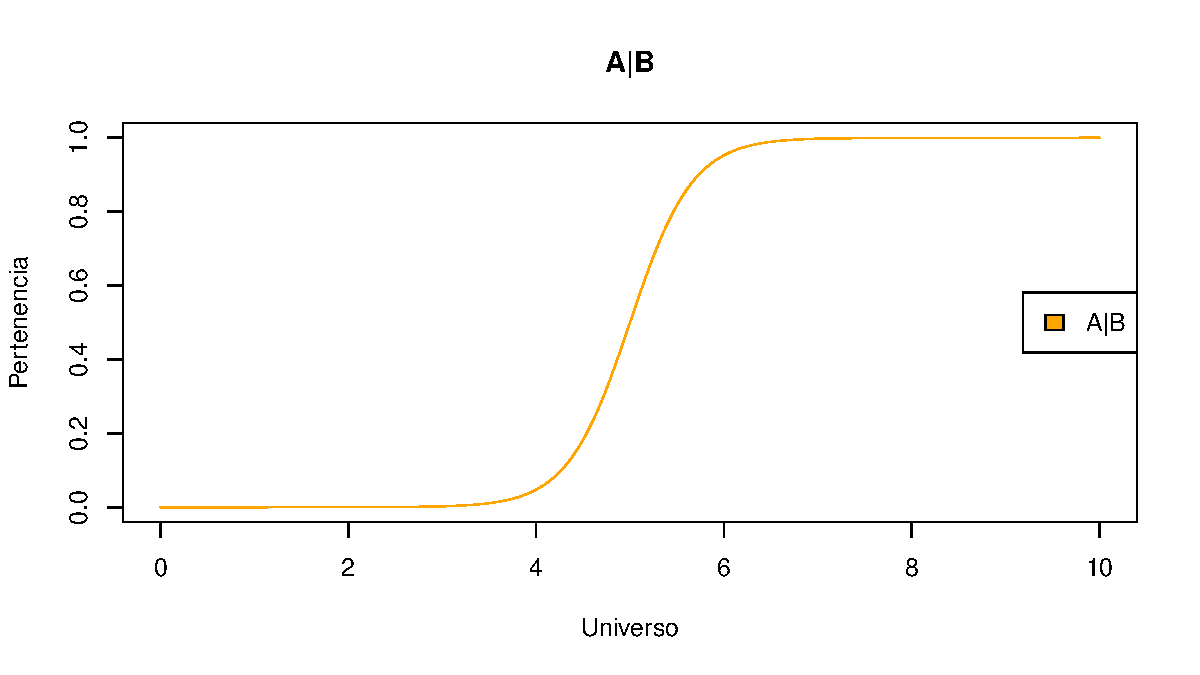
\includegraphics{tareaB3_files/figure-latex/unnamed-chunk-5-1.pdf} Para
hacerlo analíticamente, tenemos que calcular el máximo de las funciones
de pertenencia:
\[\mu_{A}\left(x\right)\geq\mu_{\overline{B}}\left(x\right)\iff\frac{1}{1+e^{-2\left(x-4\right)}}\geq\frac{1}{1+e^{-3\left(x-5\right)}}\iff-2\left(x-4\right)\geq-3\left(x-5\right)\iff\]
\[\iff x-4\leq\frac{3}{2}\left(x-5\right)\iff-\frac{x}{2}\leq\frac{-15+8}{2}=\frac{-7}{2}\iff-x\leq-7\iff x\geq7\]
Por lo tanto, es \[\mu_{A\setminus B}\left(x\right)=\begin{cases}
\mu_{\overline{B}}\left(x\right) & x\leq7\\
\mu_{A}\left(x\right) & x>7
\end{cases}\]

Y la otra diferencia es
\[\mu_{B\setminus A}\left(x\right)=\mu_{B\cap\overline{A}}\left(x\right)=\min\left\{ \mu_{B}\left(x\right),\mu_{\overline{A}}\left(x\right)\right\}\]

Que gráficamente queda:

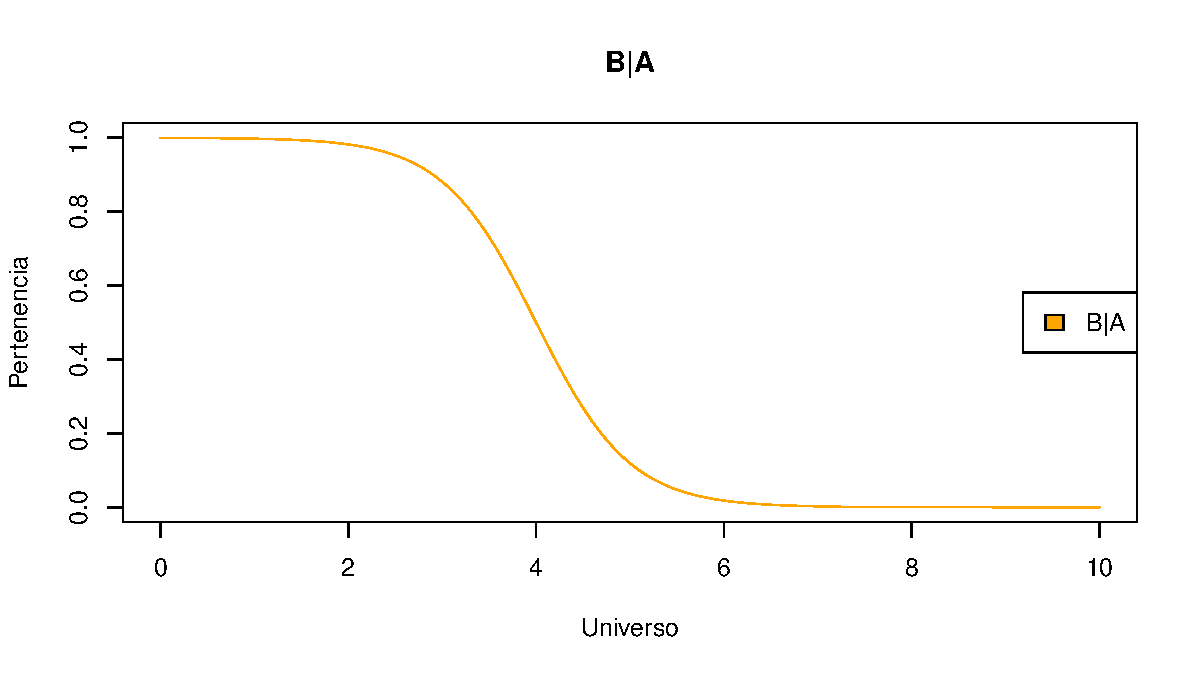
\includegraphics{tareaB3_files/figure-latex/unnamed-chunk-6-1.pdf}

Y analíticamente, igual que antes:
\[\mu_{B}\left(x\right)\geq\mu_{\overline{A}}\iff\frac{1}{1+e^{3\left(x-5\right)}}\geq\frac{1}{1+e^{2\left(x-4\right)}}\iff3\left(x-5\right)\leq2\left(x-4\right)\iff\]
\[\iff x-5\leq\frac{2}{3}\left(x-4\right)\iff\frac{x}{3}\leq\frac{7}{3}\iff x\leq7\]
por lo que la función de pertenencia es
\[\mu_{B\setminus A}\left(x\right)=\begin{cases}
\mu_{B}\left(x\right) & x\leq7\\
\mu_{\overline{A}}\left(x\right) & x>7
\end{cases}\]

Respecto a las \textbf{leyes de Morgan}, son
\[\mu_{\overline{A\cup B}}\left(x\right)=1-\mu_{A\cup B}\left(x\right)=\begin{cases}
1-\mu_{B}\left(x\right) & x\leq\frac{23}{5}\\
1-\mu_{A}\left(x\right) & x>\frac{23}{5}
\end{cases}=\begin{cases}
\mu_{\overline{B}}\left(x\right) & x\leq\frac{23}{5}\\
\mu_{\overline{A}}\left(x\right) & x>\frac{23}{5}
\end{cases}=\mu_{\overline{A}\cap\overline{B}}\] siendo cierta esta
igualdad, ya que se tiene la siguiente cadena de desigualdades
\[\mu_{\overline{B}}\left(x\right)\leq\mu_{\overline{A}}\left(x\right)\iff\frac{1}{1+e^{-3\left(x-5\right)}}\leq\frac{1}{1+e^{2\left(x-4\right)}}\iff-3\left(x-5\right)\geq2\left(x-4\right)\iff\]
\[\iff x-5\leq-\frac{2}{3}\left(x-4\right)\iff\frac{5}{3}x\leq\frac{23}{3}\iff x\leq\frac{23}{5}\]

Para la otra ley, repetimos un proceso análogo:
\[\mu_{\overline{A\cap B}}\left(x\right)=1-\mu_{A\cap B}\left(x\right)=\begin{cases}
\mu_{\overline{A}}\left(x\right) & x\leq\frac{23}{5}\\
\mu_{\overline{B}}\left(x\right) & x>\frac{23}{5}
\end{cases}=\mu_{\overline{A}\cup\overline{B}}\]

Y vemos ambas leyes gráficamente:

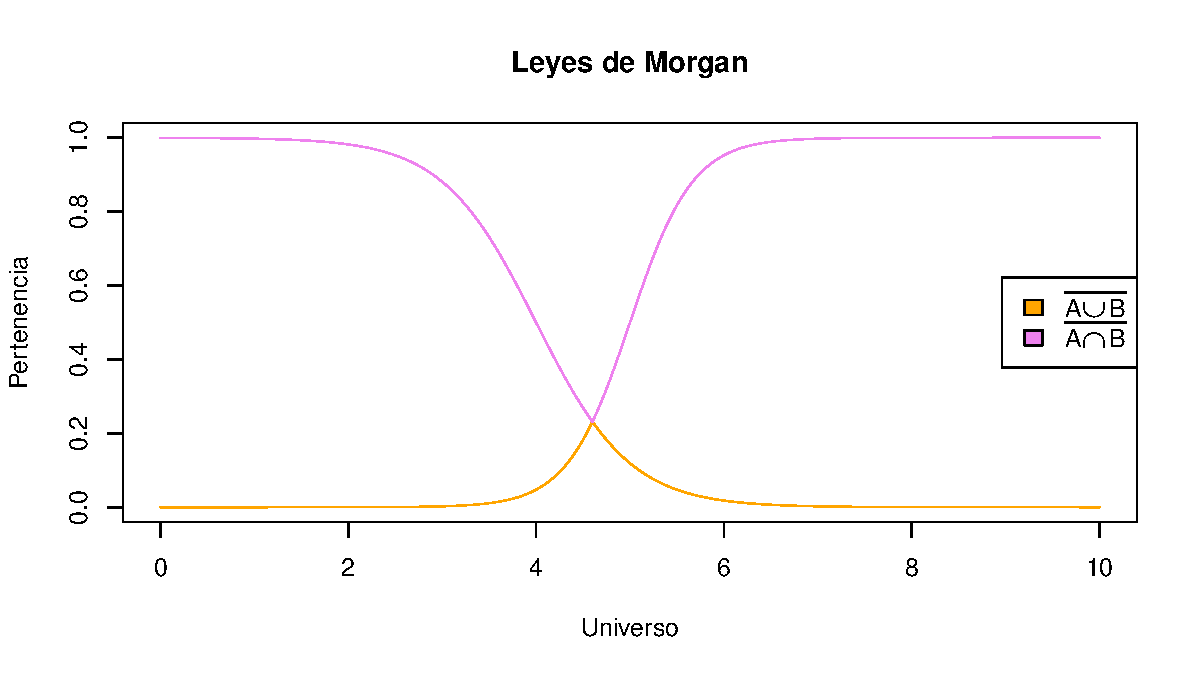
\includegraphics{tareaB3_files/figure-latex/unnamed-chunk-7-1.pdf}
Respecto a la \textbf{ley del medio excluido}:
\[\mu_{A\cap\overline{A}}\left(x\right)=\min\left\{ \mu_{A}\left(x\right),\mu_{\overline{A}}\left(x\right)\right\} \]
y se tiene que
\[\mu_{A}\left(x\right)\leq\mu_{\overline{A}}\left(x\right)\iff\frac{1}{1+e^{-2\left(x-4\right)}}\leq\frac{1}{1+e^{2\left(x-4\right)}}\iff-2\left(x-4\right)\geq2\left(x-4\right)\iff\]
\[4-x\geq x-4\iff8\geq2x\iff x\leq4\] por lo que la función de
pertenencia es \[\mu_{A\cap\overline{A}}\left(x\right)=\begin{cases}
\mu_{A}\left(x\right) & x\leq4\\
\mu_{\overline{A}}\left(x\right) & x>4
\end{cases}\]

Antes de hacerlo gráficamente, lo hacemos para el conjunto \(B\). Se
tiene la siguiente cadena de equivalencias:
\[\mu_{B}\left(x\right)\leq\mu_{\overline{B}}\left(x\right)\iff\frac{1}{1+e^{3\left(x-5\right)}}\leq\frac{1}{1+e^{-3\left(x-5\right)}}\iff3\left(x-5\right)\geq-3\left(x-5\right)\iff\]
\[\iff x-5\geq5-x\iff2x\geq10\iff x\geq5\] y entonces
\[\mu_{B\cap\overline{B}}\left(x\right)=\begin{cases}
\mu_{\overline{B}}\left(x\right) & x\leq5\\
\mu_{B}\left(x\right) & x>5
\end{cases}\]

Lo vemos gráficamente:

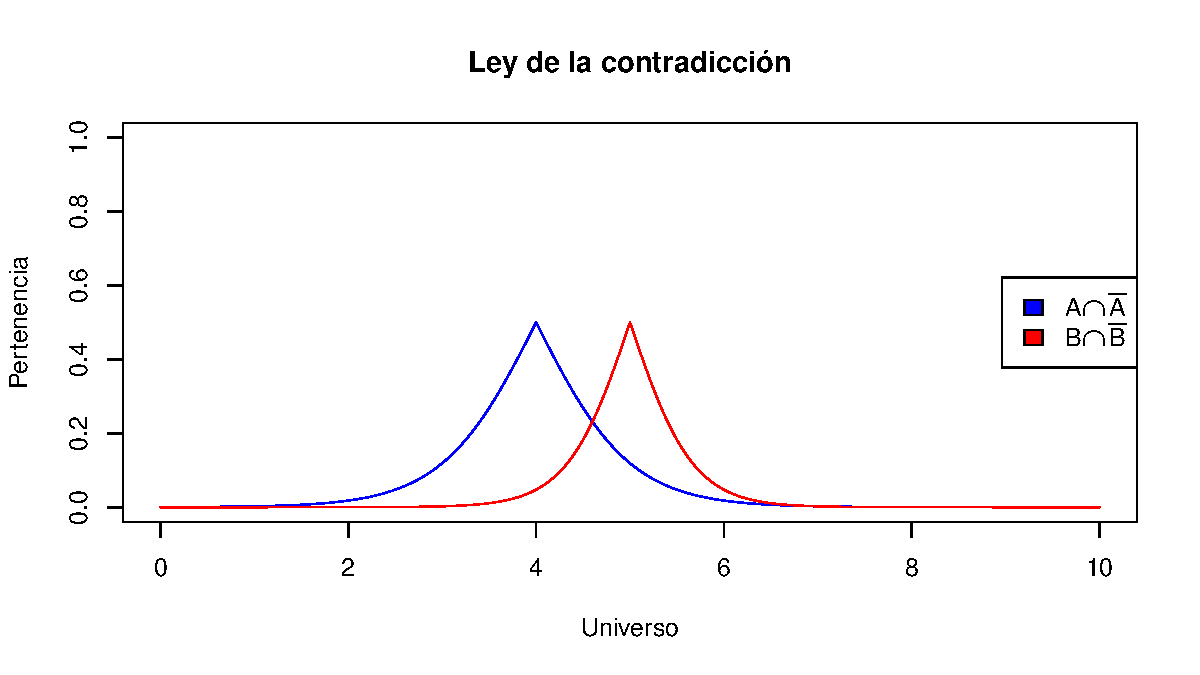
\includegraphics{tareaB3_files/figure-latex/unnamed-chunk-8-1.pdf} Por
último, abarcamos la \textbf{ley de la contradicción}:
\[\mu_{A\cup\overline{A}}\left(x\right)=\mu_{\overline{\overline{A\cup\overline{A}}}}\left(x\right)=1-\mu_{\overline{A\cup\overline{A}}}\left(x\right)=1-\mu_{\overline{A}\cap A}\left(x\right)=\begin{cases}
1-\mu_{A}\left(x\right) & x\leq4\\
1-\mu_{\overline{A}}\left(x\right) & x>4
\end{cases}=\begin{cases}
\mu_{\overline{A}}\left(x\right) & x\leq4\\
\mu_{A}\left(x\right) & x>4
\end{cases}\] Obsérvese que no es más que el complementario de la ley
del medio excluido. Para \(B\), más de lo mismo:
\[\mu_{B\cup\overline{B}}\left(x\right)=\mu_{\overline{\overline{B\cup\overline{B}}}}\left(x\right)=1-\mu_{\overline{B\cup\overline{B}}}\left(x\right)=1-\mu_{\overline{B}\cap B}\left(x\right)=\begin{cases}
1-\mu_{\overline{B}}\left(x\right) & x\leq5\\
1-\mu_{B}\left(x\right) & x>5
\end{cases}=\begin{cases}
\mu_{B}\left(x\right) & x\leq5\\
\mu_{\overline{B}}\left(x\right) & x>5
\end{cases}\]

Y vemos ambos de forma gráfica:

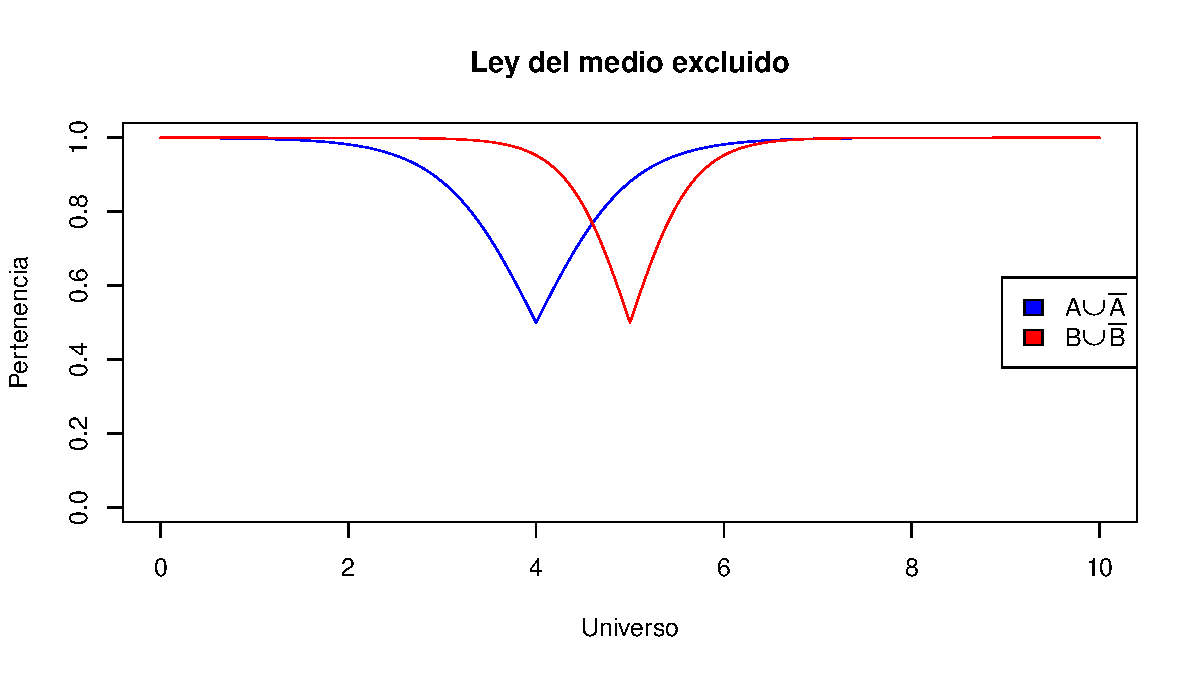
\includegraphics{tareaB3_files/figure-latex/unnamed-chunk-9-1.pdf}
\newpage

\hypertarget{problema-2}{%
\section{Problema 2}\label{problema-2}}

Supongamos que estamos diseñando un sistema para localizar objetos y
formas en una imagen. Un objeto determinado puede ser considerado grande
o pequeño, si el número de píxeles consecutivos en la matriz que
representa la imagen está por encima o por debajo de un determinado
valor. Si definimos el universo de discurso del número de píxeles
consecutivos por encima del valor de referencia como
\(\left[50,300\right]\), podemos definir los siguientes conjuntos
borrosos:
\["Grande"=\left\{ \frac{0}{50}+\frac{0.2}{100}+\frac{0.3}{150}+\frac{0.8}{200}+\frac{0.9}{250}+\frac{1}{300}\right\} \]
\["Pequeño"=\left\{ \frac{1}{50}+\frac{0.5}{100}+\frac{0.1}{150}+\frac{0}{200}+\frac{0}{250}+\frac{0}{300}\right\} \]
donde las distintas formas detectadas se pueden expresar en los
siguientes términos:

\begin{enumerate}
\def\labelenumi{\arabic{enumi}.}
\item
  Muy grande
\item
  Más que muy grande
\item
  No muy grande y más o menos pequeño
\item
  Muy muy grande y no pequeño
\item
  Muy pequeño y no grande
\item
  Bastante grande (=grande\(^{\frac{2}{3}}\))
\item
  Ni muy pequeño ni muy grande
\item
  Pequeño o no muy pequeño
\end{enumerate}

Calcular las funciones de pertenencia para cada uno de los términos
anteriores.

Vamos a calcular las funciones de pertenencia tal y como se definen en
los apuntes de clase
~{[}\protect\hyperlink{ref-PalmaLogicaBorrosa}{3}{]}. De esta manera, y
teniendo en cuenta que \[\mu_{Grande}\left(x\right)=\begin{cases}
0 & x=50\\
0.2 & x=100\\
0.3 & x=150\\
0.8 & x=200\\
0.9 & x=250\\
1 & x=300
\end{cases}\quad \mu_{Pequeño}\left(x\right)=\begin{cases}
1 & x=50\\
0.5 & x=100\\
0.1 & x=150\\
0 & x=200\\
0 & x=250\\
0 & x=300
\end{cases}\] sería:

\begin{enumerate}
\def\labelenumi{\arabic{enumi}.}
\item
  Muy grande:
  \[\mu_{MUY\ Grande}\left(x\right)=\mu_{Grande}\left(x\right)^{2}=\begin{cases}
  0 & x=50\\
  0.04 & x=100\\
  0.09 & x=150\\
  0.64 & x=200\\
  0.81 & x=250\\
  1 & x=300
  \end{cases}\]
\item
  Más que muy grande:
  \[\mu_{MAS\ MUY\ Grande}\left(x\right)=\mu_{MUY\ Grande}\left(x\right)^{1.25}=\begin{cases}
  0 & x=50\\
  0.01788854 & x=100\\
  0.04929503 & x=150\\
  0.5724334 & x=200\\
  0.7684335 & x=250\\
  1 & x=300
  \end{cases}\]
\item
  No muy grande y más o menos pequeño: este caso tiene un poco más de
  complejidad. Primero, hacemos `no muy grande':
  \[\mu_{NO\ MUY\ Grande}\left(x\right)=1-\mu_{MUY\ Grande}\left(x\right)=\begin{cases}
  1 & x=50\\
  0.96 & x=100\\
  0.91 & x=150\\
  0.36 & x=200\\
  0.09 & x=250\\
  0 & x=300
  \end{cases}\] Ahora hacemos `más o menos pequeño':
  \[\mu_{MASMENOS\ Pequeño}\left(x\right)=\mu_{Pequeño}\left(x\right)^{\frac{1}{2}}=\begin{cases}
  1 & x=50\\
  0.7071068 & x=100\\
  0.3162278 & x=150\\
  0 & x=200\\
  0 & x=250\\
  0 & x=300
  \end{cases}\] Y lo pedido por el enunciado es su intersección, o sea,
  el mínimo de las funciones de pertenencia:
  \[\mu_{NO\ MUY\ Grande\ Y\ MASMENOS\ Pequeño}\left(x\right)=\min\left\{ \mu_{NO\ MUY\ Grande}\left(x\right),\mu_{MASMENOS\ Pequeño}\left(x\right)\right\} =\]
  \[=\begin{cases}
  1 & x=50\\
  0.7071068 & x=100\\
  0.3162278 & x=150\\
  0 & x=200\\
  0 & x=250\\
  0 & x=300
  \end{cases}=\mu_{MASMENOS\ Pequeño}\left(x\right)\] observamos que
  coincide con la función de pertenencia de `más o menos pequeño.'
\item
  Muy muy grande y no pequeño: de nuevo, calculamos cada una por
  separado y después las juntamos tomando el mínimo:
  \[\mu_{MUY\ MUY\ Grande}\left(x\right)=\mu_{MUY\ Grande}\left(x\right)^{2}=\begin{cases}
  0 & x=50\\
  0.0003199999 & x=100\\
  0.00243 & x=150\\
  0.32768 & x=200\\
  0.59049 & x=250\\
  1 & x=300
  \end{cases}\]
  \[\mu_{NO\ Pequeño}\left(x\right)=1-\mu_{Pequeño}\left(x\right)=\begin{cases}
  0 & x=50\\
  0.5 & x=100\\
  0.9 & x=150\\
  1 & x=200\\
  1 & x=250\\
  1 & x=300
  \end{cases}\] y tomando el mínimo es:
  \[\mu_{MUY\ MUY\ Grande\ Y\ NO\ Pequeño}\left(x\right)=\begin{cases}
  0 & x=50\\
  0.0003199999 & x=100\\
  0.00243 & x=150\\
  0.32768 & x=200\\
  0.59049 & x=250\\
  1 & x=300
  \end{cases}=\mu_{MUY\ MUY\ Grande}\left(x\right)\] Que coincide con
  ser `muy muy grande.'
\item
  Muy pequeño y no grande:
  \[\mu_{MUY\ Pequeño}\left(x\right)=\begin{cases}
  1 & x=50\\
  0.25 & x=100\\
  0.01 & x=150\\
  0 & x=200\\
  0 & x=250\\
  0 & x=300
  \end{cases} \qquad \mu_{NO\ Grande}\left(x\right)=\begin{cases}
  1 & x=50\\
  0.8 & x=100\\
  0.7 & x=150\\
  0.2 & x=200\\
  0.1 & x=250\\
  0 & x=300
  \end{cases}\]
\end{enumerate}

Y entonces
\[\mu_{MUY\ Pequeño\ Y\ NO\ Grande}\left(x\right)=\begin{cases}
1 & x=50\\
0.25 & x=100\\
0.01 & x=150\\
0 & x=200\\
0 & x=250\\
0 & x=300
\end{cases}=\mu_{MUY\ Pequeño}\left(x\right)\]

\begin{enumerate}
\def\labelenumi{\arabic{enumi}.}
\setcounter{enumi}{5}
\item
  Bastante grande: tal y como indica el enunciado, es
  \[\mu_{BASTANTE\ Grande}\left(x\right)=\mu_{Grande}\left(x\right)^{\frac{2}{3}}=\begin{cases}
  0 & x=50\\
  0.3419952 & x=100\\
  0.4481405 & x=150\\
  0.8617739 & x=200\\
  0.9321698 & x=250\\
  1 & x=300
  \end{cases}\]
\item
  Ni muy pequeño ni muy grande: esto es lo mismo que decir `no muy
  pequeño y no muy grande,' por lo que calculamos:
  \[\mu_{NO\ MUY\ Pequeño}\left(x\right)=\begin{cases}
  0 & x=50\\
  0.75 & x=100\\
  0.99 & x=150\\
  1 & x=200\\
  1 & x=250\\
  1 & x=300
  \end{cases} \quad \mu_{NO\ MUY\ Grande}\left(x\right)=\begin{cases}
  1 & x=50\\
  0.96 & x=100\\
  0.91 & x=150\\
  0.36 & x=200\\
  0.19 & x=250\\
  0 & x=300
  \end{cases}\] y su intersección queda:
  \[\mu_{NO\ MUY\ Pequeño\ Y\ NO\ MUY\ Grande}\left(x\right)=\begin{cases}
  0 & x=50\\
  0.75 & x=100\\
  0.91 & x=150\\
  0.36 & x=200\\
  0.19 & x=250\\
  0 & x=300
  \end{cases}\]
\item
  Pequeño o no muy pequeño: en este caso debemos tomar el máximo, y las
  dos funciones de pertenencia involucradas ya las conocemos:
  \[\mu_{Pequeño\ O\ NO\ MUY\ Pequeño}\left(x\right)=\max\left\{ \mu_{Pequeño}\left(x\right),\mu_{NO\ MUY\ Pequeño}\left(x\right)\right\} =\begin{cases}
  1 & x=50\\
  0.75 & x=100\\
  0.99 & x=150\\
  1 & x=200\\
  1 & x=250\\
  1 & x=300
  \end{cases}\]
\end{enumerate}

\newpage

\hypertarget{problema-3}{%
\section{Problema 3}\label{problema-3}}

Queremos desarrollar un sistema controlador para regular la temperatura
de una habitación. Una vez analizado el problema, hemos llegado a la
conclusión de que solo con una regla podemos alcanzar el objetivo:
``Cuando la habitación está caliente, endría la habitación activando el
ventilador a una velocidad alta.'' Es decir, podemos codiifcar el
funcionamiento del controlador con la regla:

\[\boldsymbol{SI}\ la\ temperatura\ es\ ALTA\ \boldsymbol{ENTONCES}\ la\ velocidad\ de\ giro\ tiene\ que\ ser\ \boldsymbol{RÁPIDA}\]

Para utilizar esta regla se definen los conjuntos borrosos ``Temperatura
alta,'' \(C\), sobre el universo formado por las temperaturas en ºC, y
el conjunto ``rápida,'' sobre el universo de velocidades de giro en 1000
rpm:

\[C="Temperatura\ alta"=\left\{ \frac{0.0}{16}+\frac{0.1}{20}+\frac{0.7}{25}+\frac{0.9}{30}+\frac{1.0}{35}\right\} \]
\[R="rápida"=\left\{ \frac{0.0}{0}+\frac{0.2}{1}+\frac{0.5}{2}+\frac{0.9}{3}+\frac{1.0}{4}\right\} \]

\begin{enumerate}
\def\labelenumi{\arabic{enumi}.}
\item
  Para los anteriores conjuntos borrosos construir la relación de
  implicación utilizando:

  \begin{itemize}
  \item
    La interpretación clásica de la implicación
  \item
    La implicación de Mandami
  \item
    La implicación de Larsen
  \item
    Comparar los anteriores resultados
  \end{itemize}
\item
  Supongamos que modificamos el antecedente de la regla introduciendo el
  siguiente conjunto borroso:
  \[C'="Moderadamente\ alta"=\left\{ \frac{0.0}{16}+\frac{0.2}{20}+\frac{1.0}{30}+\frac{1.0}{35}\right\} \]
  calcular el conjunto borroso que describe la velocidad del ventilador
  utilizando:

  \begin{itemize}
  \item
    La composición max-min para las implicaciones clásica y Mandami
  \item
    La composición max-producto para la implicación Larsen
  \item
    En el caso de las implicaciones de Mandami y Larsen utiliza la
    expresión basada en el grado de satisfacción
  \end{itemize}
\item
  Supongamos que modificamos el consecuente de la regla introduciendo el
  siguiente conjunto borroso:
  \[R'="Moderamente\ rápida"=\left\{ \frac{0.0}{0}+\frac{0.4}{1}+\frac{0.7}{2}+\frac{1.0}{3}+\frac{1.0}{4}\right\} \]
  calcular el conjunto borroso que describe la temperatura de la
  habitación utilizando:

  \begin{itemize}
  \item
    La composición max-min para las implicaciones clásica y Mandami
  \item
    La composición max-producto para la implicación Larsen
  \end{itemize}
\end{enumerate}

Empecemos por el principio:

\begin{enumerate}
\def\labelenumi{\arabic{enumi}.}
\item
  Tal y como se explica en
  ~{[}\protect\hyperlink{ref-BotiaPalmaImplicaciones}{4}{]} o en
  ~{[}\protect\hyperlink{ref-PalmaLogicaBorrosa}{3}{]}, la implicación
  clásica es la de Dienes-Rescher, y consiste en interpretar
  \(p\rightarrow q\) como \(\neg p\lor q\). Por lo tanto,
  \[I_{Clasica}\left(c,r\right)=\mu_{C\rightarrow R}\left(c,r\right)=\max\left\{ 1-\mu_{C}\left(c\right),\mu_{R}\left(r\right)\right\} \]
  y entonces, la relación borrosa resultante es:
  \[\widetilde{R_{Clasica}}=\begin{array}{cccccc}
   & 0 & 1 & 2 & 3 & 4\\
  16 & 1 & 1 & 1 & 1 & 1\\
  20 & 0.9 & 0.9 & 0.9 & 0.9 & 1\\
  25 & 0.3 & 0.3 & 0.5 & 0.9 & 1\\
  30 & 0.1 & 0.2 & 0.5 & 0.9 & 1\\
  35 & 0 & 0.2 & 0.5 & 0.9 & 1
  \end{array}\] La implicación de Mandani es la que responde a la
  fórmula:
  \[I_{M}\left(c,r\right)=\mu_{C\rightarrow R}\left(c,r\right)=\min\left\{ \mu_{C}\left(c\right),\mu_{R}\left(r\right)\right\} \]
  por lo que obtenemos la relación borrosa:
  \[\widetilde{R_{M}}=\begin{array}{cccccc}
   & 0 & 1 & 2 & 3 & 4\\
  16 & 0 & 0 & 0 & 0 & 0\\
  20 & 0 & 0.1 & 0.1 & 0.1 & 0.1\\
  25 & 0 & 0.2 & 0.5 & 0.7 & 0.7\\
  30 & 0 & 0.2 & 0.5 & 0.9 & 0.9\\
  35 & 0 & 0.2 & 0.5 & 0.9 & 1
  \end{array}\] Respecto a la implicación de Larsen, es la
  correspondiente a la t-norma del producto:
  \[I_{L}\left(c,r\right)=\mu_{C\rightarrow R}\left(c,r\right)=\mu_{C}\left(r\right)\cdot\mu_{R}\left(r\right)\]
  que nos da la siguiente relación:
  \[\widetilde{R_{L}}=\begin{array}{cccccc}
   & 0 & 1 & 2 & 3 & 4\\
  16 & 0 & 0 & 0 & 0 & 0\\
  20 & 0 & 0.01 & 0.1 & 0.1 & 0.1\\
  25 & 0 & 0.14 & 0.35 & 0.63 & 0.7\\
  30 & 0 & 0.18 & 0.45 & 0.81 & 0.9\\
  35 & 0 & 0.2 & 0.5 & 0.9 & 1
  \end{array}\] Como puede observarse, se verifica que
  \(\widetilde{R_{L}}\left(c,r\right)\leq\widetilde{R_{M}}\left(c,r\right)\leq\widetilde{R_{Clasica}}\left(c,r\right),\forall c\in C,\forall r\in R\).
  Esto sucede siempre entre estos tres modelos de implicaciones, por la
  desigualdad general
  \[a\cdot b\leq\min\left\{ a,b\right\} \leq\max\left\{ a,b\right\} ,\ \forall a,b\in\left[0,1\right]\]
  y se traduce en que, a la hora de hacer inferencia, la implicación de
  Larsen proporcionará un conjunto borroso con una función de
  pertenencia menor o igual que la obtenida al usar Mandani, y esta, a
  su vez, será menor que la obtenida con la implicación clásica.
\item
\end{enumerate}

\newpage

\hypertarget{problema-4}{%
\section{Problema 4}\label{problema-4}}

Se nos ha pedido diseñar un sistema de inferencia borroso para simular
el descenso final y las maniobras de aterrizaje de un avión. La
velocidad de descenso es proporcional al cuadrado de la altitud. De esta
forma, para altitudes grandes se requiere una velocidad de descenso
grande. A medida que la altitud disminuye, la velocidad de descenso va
disminuyendo. En el límite, la altitud se hará infinitamente pequeña y
la velocidad tenderá a ceor. De esta forma el avión descenderá
bruscamente pero aterrizará suavemente para evitar daños.

Las dos variables de estado para esta simulación son la altitud, h, y la
velocidad de descenso, v. La variable de control obtenida como salida
del SIB será la fuerza que, una vez aplicada al avión, modificará su
altitud h, y su velocidad v. Para el diseño del controlador borroso se
han definido las siguientes variables lingüísticas:

\begin{itemize}
\tightlist
\item
  \textbf{Altitud}, definida sobre el universo de discurso
  \(X_{1}=\left[0,1000\right]\) (en pies), a través de los siguientes
  conjuntos borrosos:
\end{itemize}

\[Grande\left(L\right)=\mu_{L}\left(x\right)=\left\{ \frac{0}{500}+\frac{0.2}{600}+\frac{0.4}{700}+\frac{0.6}{800}+\frac{0.8}{900}+\frac{1}{1000}\right\} \]
\[Media\left(M\right)=\mu_{M}\left(x\right)=\left\{ \frac{0}{300}+\frac{0.2}{400}+\frac{0.4}{500}+\frac{0.6}{600}+\frac{0.8}{700}+\frac{1}{800}+\frac{0.8}{900}+\frac{0.6}{1000}\right\} \]
\[Pequeña\left(S\right)=\mu_{S}\left(x\right)=\left\{ \frac{0.4}{0}+\frac{0.6}{100}+\frac{0.8}{200}+\frac{1}{300}+\frac{0.8}{400}+\frac{0.6}{500}+\frac{0.4}{600}+\frac{0.2}{700}+\frac{0}{800}\right\} \]
\[Cerca\_cero\left(NZ\right)=\mu_{NZ}\left(x\right)=\left\{ \frac{1}{0}+\frac{0.8}{100}+\frac{0.6}{200}+\frac{0.4}{300}+\frac{0.2}{400}+\frac{0}{500}\right\} \]

\begin{itemize}
\tightlist
\item
  \textbf{Velocidad}, definida sobre el universo
  \(X_{2}=\left[-30,30\right]\) (pies/seg) a través de los siguientes
  conjuntos borrosos:
\end{itemize}

\[alta\ ascendente\left(UL\right)=\mu_{UL}\left(x\right)=\left\{ \frac{0}{10}+\frac{0.5}{15}+\frac{1}{20}+\frac{1}{25}+\frac{1}{30}\right\} \]
\[baja\ ascendente\left(US\right)=\mu_{US}\left(x\right)=\left\{ \frac{0}{0}+\frac{0.5}{5}+\frac{1}{10}+\frac{0.5}{15}+\frac{0}{20}\right\} \]
\[cero\left(Z\right)=\mu_{Z}\left(x\right)=\left\{ \frac{0}{-10}+\frac{0.5}{-5}+\frac{1}{0}+\frac{0.5}{5}+\frac{0}{10}\right\} \]
\[baja\ descendente\left(DS\right)=\mu_{DS}\left(x\right)=\left\{ \frac{0}{-20}+\frac{0.5}{-15}+\frac{1}{-10}+\frac{0.5}{-5}+\frac{0}{0}\right\} \]
\[alta\ ascendente\left(DL\right)=\mu_{DL}\left(x\right)=\left\{ \frac{1}{-30}+\frac{1}{-25}+\frac{1}{-20}+\frac{0.5}{-15}+\frac{0}{-10}\right\} \]

\begin{itemize}
\tightlist
\item
  \textbf{Fuerza de control}, definida sobre el universo
  \(X_{3}=\left[-30,30\right]\) (libras), a través de los siguientes
  conjuntos borrosos:
\end{itemize}

\[alta\ ascendente\left(UL\right)=\mu_{UL}\left(x\right)=\left\{ \frac{0}{10}+\frac{0.5}{15}+\frac{1}{20}+\frac{1}{25}+\frac{1}{30}\right\} \]
\[baja\ ascendente\left(US\right)=\mu_{US}\left(x\right)=\left\{ \frac{0}{0}+\frac{0.5}{5}+\frac{1}{10}+\frac{0.5}{15}+\frac{0}{20}\right\} \]
\[cero\left(Z\right)=\mu_{Z}\left(x\right)=\left\{ \frac{0}{-10}+\frac{0.5}{-5}+\frac{1}{0}+\frac{0.5}{5}+\frac{0}{10}\right\} \]
\[baja\ descendente\left(DS\right)=\mu_{DS}\left(x\right)=\left\{ \frac{0}{-20}+\frac{0.5}{-15}+\frac{1}{-10}+\frac{0.5}{-5}+\frac{0}{0}\right\} \]
\[alta\ ascendente\left(DL\right)=\mu_{DL}\left(x\right)=\left\{ \frac{1}{-30}+\frac{1}{-25}+\frac{1}{-20}+\frac{0.5}{-15}+\frac{0}{-10}\right\} \]

y el siguiente conjunto de reglas:

\begin{itemize}
\item
  \textbf{REGLA-1}: \textbf{Si} la altitud es \textbf{muy grande y} la
  velocidad es \textbf{muy alta ascendente entonces} la fuerza debe ser
  \textbf{alta descendente}
\item
  \textbf{REGLA-2}: \textbf{Si} la altitud es \textbf{media y} la
  velocidad es \textbf{baja ascendente entonces} la fuerza debe ser
  \textbf{baja descendente}
\item
  \textbackslash textbf\{REGLA-3: \textbf{Si} la altitud es
  \textbf{algo media y} la velocidad es
  \textbf{algo alta ascendente entonces} la fuerza debe ser
  \textbf{baja descendente}
\item
  \textbackslash textbf\{REGLA-4: \textbf{Si} la altitud es
  \textbf{pequeña y} la velocidad es \textbf{baja descendente entonces}
  la fuerza debe ser \textbf{baja ascendente}
\item
  \textbackslash textbf\{REGLA-5: \textbf{Si} la altitud es
  \textbf{cercana a cero o} la velocidad es \textbf{cero entonces} la
  fuerza debe ser \textbf{cero}
\item
  \textbackslash textbf\{REGLA-6: \textbf{Si} la altitud \textbf{no} es
  \textbf{cercana a cero} y la velocidad \textbf{no} es \textbf{cero}
  entonces la fuera debe ser \textbf{baja descendente}
\end{itemize}

Se pide:

\begin{enumerate}
\def\labelenumi{\arabic{enumi}.}
\tightlist
\item
  Determinar las salidas del sistema de inferencia borroso para un avión
  con una altitud de 700fts y una velocidad de 15 fts/s utilizando, el
  fuzzificador unitario y:

  \begin{enumerate}
  \def\labelenumii{\alph{enumii}.}
  \tightlist
  \item
    El operador implicación de Mandani
  \item
    El operador implicación de Larsen
  \end{enumerate}
\item
  Defuzzificar el resultado utilizando la técnica del centroide
\end{enumerate}

\newpage

\hypertarget{problema-5}{%
\section{Problema 5}\label{problema-5}}

El problema de simulación del aterrizaje de los aviones descrito
anteriormente nos permitía obtener la fuerza que hay que aplicarle al
avión dada una altitud y velocidad determinadas. Una vez determinada la
fuerza, la nueva velocidad y altitud se calculan mediante las siguientes
expresiones: \[v_{i+1}=v_{i}+f_{i}\] \[h_{i+1}=h_{i}+v_{i}\] donde
\(v_{i+1}\) y \(h_{i+1}\) son la nueva velocidad y altitud
respectivamente una vez apicada una fuerza \(f_{i}\) a un avión con una
altitud \(h_{i}\) y una velocidad de descenso \(v_{i}\), siendo
\(v_{0}\) y \(h_{0}\) los valores iniciales de velocidad y altitud. Se
pide:

\begin{enumerate}
\def\labelenumi{\arabic{enumi}.}
\item
  Partiendo del sistema definido en el apartado anterior, y para los
  mismos valores de entrada, resolver con JFuzzyLogic el problema
  anterior para los mismos valores de entrada, pero sustituyendo el
  conjunto de reglas por las siguientes reglas:

  \begin{table}[H]
  \centering
  \begin{tabular}{|l|llllll|}
  \hline
                                 & \multicolumn{6}{l|}{\textbf{Velocidad de descenso}}                                                                                                                                       \\ \hline
  \multirow{5}{*}{\textbf{Altitud}} & \multicolumn{1}{l|}{}            & \multicolumn{1}{l|}{\textbf{DL}} & \multicolumn{1}{l|}{\textbf{DS}} & \multicolumn{1}{l|}{\textbf{Z}} & \multicolumn{1}{l|}{\textbf{US}} & \textbf{UL} \\ \cline{2-7} 
                                 & \multicolumn{1}{l|}{\textbf{L}}  & \multicolumn{1}{l|}{Z}           & \multicolumn{1}{l|}{DS}          & \multicolumn{1}{l|}{DL}         & \multicolumn{1}{l|}{DL}          & DL          \\ \cline{2-7} 
                                 & \multicolumn{1}{l|}{\textbf{M}}  & \multicolumn{1}{l|}{US}          & \multicolumn{1}{l|}{Z}           & \multicolumn{1}{l|}{DS}         & \multicolumn{1}{l|}{DL}          & DL          \\ \cline{2-7} 
                                 & \multicolumn{1}{l|}{\textbf{S}}  & \multicolumn{1}{l|}{UL}          & \multicolumn{1}{l|}{US}          & \multicolumn{1}{l|}{Z}          & \multicolumn{1}{l|}{DS}          & DL          \\ \cline{2-7} 
                                 & \multicolumn{1}{l|}{\textbf{NZ}} & \multicolumn{1}{l|}{UL}          & \multicolumn{1}{l|}{UL}          & \multicolumn{1}{l|}{Z}          & \multicolumn{1}{l|}{DS}          & DS          \\ \hline
  \end{tabular}
  \end{table}

  Adjuntar las imágenes en las que se puedan apreciar cómo están
  definidas las diferentes variables borrosas y el resultado de la
  evaluación de las reglas.
\item
  Realizar una aplicación, utilizando JFuzzyLogic, que realice la
  simulación del aterrizaje del avión. Para ello nos basaremos en el SIB
  definido a aprtir de las reglas del apartado anterior y de las
  ecuaciones de estado indicadas al comienzo del problema. Considerar
  que los incrementos de tiempos son de un segundo.
\item
  El resultado de la simulación se puede presentar de la siguiente
  forma:

  \begin{enumerate}
  \def\labelenumii{\alph{enumii}.}
  \item
    A través del terminal de eclipse imprimiendo en cada línea la
    evolución de cada parámetro
  \item
    Mediante gráficas que muestren la evolución de los parámetros
  \item
    Mediante simulación animada del proceso de aterrizaje
  \end{enumerate}
\end{enumerate}

\newpage

\hypertarget{bibliografuxeda}{%
\section{Bibliografía}\label{bibliografuxeda}}

\hypertarget{refs}{}
\begin{CSLReferences}{0}{0}
\leavevmode\hypertarget{ref-PalmaConjuntosBorrosos}{}%
\CSLLeftMargin{{[}1{]} }
\CSLRightInline{J. T. Palma, \emph{Conjuntos Borrosos}, (2013).}

\leavevmode\hypertarget{ref-BotiaConjuntosBorrosos}{}%
\CSLLeftMargin{{[}2{]} }
\CSLRightInline{J. A. Botia, \emph{Ejercicios Ejemplo de Conjuntos
Borrosos}, (2021).}

\leavevmode\hypertarget{ref-PalmaLogicaBorrosa}{}%
\CSLLeftMargin{{[}3{]} }
\CSLRightInline{J. T. Palma, \emph{Logica e Inferencia Borrosos},
(2017).}

\leavevmode\hypertarget{ref-BotiaPalmaImplicaciones}{}%
\CSLLeftMargin{{[}4{]} }
\CSLRightInline{J. T. P. Juan A. Botia, \emph{Tipos de Implicaciones y
DOF}, (2020).}

\end{CSLReferences}

\end{document}
